\documentclass[output=paper]{langsci/langscibook} 
\title{The development of finite verbs from nominalized structures in Northern Mao} 
\author{%
 Michael Ahland \affiliation{California State University, Long Beach}
}
% \chapterDOI{} %will be filled in at production
\shorttitlerunninghead{Finite verbs from nominalized structures in Northern Mao}

\abstract{Northern Mao, an endangered Omotic-Mao language of Ethiopia, exhibits rigid OV patterns where final verbs are the most finite structures in the language. Only final verbs carry tense markers and indicate the completion of a sentence. Some final verb constructions, however, display internal structural relics that attest to a nominalized heritage: infinitive verb stems and morphological subordinators. This paper examines infinitival and subordinate structures and explores the diachronic pathways which likely led to today's finite final verb forms.}

\maketitle
\begin{document}
\todo{Original title is too long for the header. Please check the shortened title in header}
\section{Introduction}
%fix citations throughout and in bibliography
Northern Mao (NM), also known by the autonym Màwés Aats'è, is an endangered Omotic-Mao language of Ethiopia \citep{Bender2000} spoken by an estimated 2-3,000 speakers \citep[13]{Ahland2012}. NM exhibits rigid OV patterns where final verbs are the most finite structures in the language. The final declarative and interrogative verbs are the only structures which express a morphologically marked tense distinction (future /-gà/ vs. non-future /-${\emptyset}$/ on irrealis verbs), and the final verbs are the only structures which indicate the completion of a full sentence (also expressed by a speech act marker on final verbs). Some final verb constructions, however, display internal structural relics which attest to a nominalized heritage. These relics include infinitive verb stems, the inclusion of a relativizer, and other subordinators. That nominalizations such as these can serve as sources for finite constructions is widely attested in the world's languages (\citealt{Gildea1993}; \citealt{DeLancey2011}; \citealt[68]{Givon2009}; \citealt[382]{Noonan1997}). This paper explores NM's infinitival and subordinate structures and offers a coherent, cross-constructional analysis of the diachronic pathways through which nominal structures were transformed into today's finite final verb forms.

The discussion begins with pertinent background information including a typological overview \sectref{sec:mahland:1.1}, a discussion of finiteness in NM \sectref{sec:mahland:1.2}, the role of tone as a marker of stem finiteness \sectref{sec:mahland:1.3}, and the nominal status of infinitive stems \sectref{sec:mahland:1.4}. The discussion then details how subordination in NM involves nominalization through an exploration of the role of infinitive stems in complement and adverbial constructions \sectref{sec:mahland:2.1}, relativization \sectref{sec:mahland:2.2}, and the /-gàʃ/ subordinator constructions \sectref{sec:mahland:2.3}. \sectref{sec:mahland:3} illustrates the indications of nominalization and subordination in main clause structures: the use of the infinitive stem in finite final verbs \sectref{sec:mahland:3.1}, the role of relativization in the past progressive construction \sectref{sec:mahland:3.2}, and the historical development of the irrealis future verb construction from an old periphrastic subordinate + final verb construction \sectref{sec:mahland:3.3}. The discussion concludes with a summary of the evidence supporting a nominalized source for finite structures. 

\subsection{Typological overview}\label{sec:mahland:1.1}

NM, like most Omotic languages, exhibits a rigid OV pattern across syntactic constructions. \tabref{tab:mahland:1} lists the NM constituent-order patterns attested relative to \cite{Greenberg1963}'s universals. 

\begin{table}
\caption{Constituent order typology of Northern Mao (from \citealt[48]{Ahland2012})}
\label{tab:mahland:1}
  	\centering
\begin{tabularx}{\textwidth}{XXX}
\lsptoprule
Greenberg's universal & Parameter & Northern Mao pattern\\
\midrule
1 & main clause & OV\\
3, 4 & adposition & NP - postposition \\
2 & genitive (possessor) and head noun & Genitive - N\\
17 & modifier and head noun & Modifier - N\\
24 &  relative clause\index{subordination!relative clauses} and head noun & Relative Clause - N\\
22 & comparatives & Standard-Marker-Quality\\
16 & inflected auxiliaries & sentence final\\
9 & question particles & sentence final\\
12 & question words & sentence initial or \textit{in situ}\\
27 & affixes & primarily suffixes\\
\lspbottomrule
\end{tabularx}
\end{table}

Examples \REF{ex:mahland:1}-\REF{ex:mahland:4} illustrate selected patterns from \tabref{tab:mahland:1}: the order of major constituents in the transitive construction \REF{ex:mahland:1}, the order of NP and adpositional element (postposition) \REF{ex:mahland:2}-\REF{ex:mahland:3}, and the order of relative clause and head noun \REF{ex:mahland:4}. 

\ea\label{ex:mahland:1}
\gll  múnts'-ìʃ       ʃóːʃ-nà          ha-pí-{\downstep}á \\
woman\textsc{{}-sbj}    snake\textsc{{}-obj}     \textsc{aff}-kill\textsc{{}-decl} \\
\glt `A woman killed a snake.'
\z        

\ea\label{ex:mahland:2}
\gll tí-ŋ           {\downstep}kjat'-èt        háːl-{\downstep}á\\
1\textsc{sg}{}-\textsc{gen}   house-\textsc{loc}   sleep-\textsc{decl} \\
\glt `S/he slept at my house.'
\z

\ea\label{ex:mahland:3}
\gll bàmbàs-ʃál-èt                 ha-tí-kí-{\downstep}á  \\
Bambassi\index{Bambassi}{}-way-\textsc{source}    \textsc{aff}{}-1\textsc{sg}{}-come-\textsc{decl}\\
\glt `I came from Bambassi\index{Bambassi}.'
\z

\ea\label{ex:mahland:4}
\gll hez-ít           mùnts'-òl-ìʃ      nók-and-wé-jà\\
hit:\textsc{inf-rel}   woman-\textsc{pl-sbj}  be.good:\textsc{inf-nsg-neg-cop}\\
\glt `Women who hit are not good.'
\z

\subsection{Finiteness in Northern Mao}\label{sec:mahland:1.2}

Finiteness in NM is scalar; it is best viewed as matter of degree where constructions can be arranged on a continuum. This view of finiteness is in accord with Givón, who defines \textit{finiteness} as ``an aggregate feature of clauses'' which involves properties of clauses as well as verbs (i.e. the licensing of arguments and other morphological structures such as case markers, and verbal inflectional morphology: subject marking, tense, aspect, modality, etc.) \citep[25]{Givon2001-2}. In NM, as is common in other OV systems, final verbs are the most finite structures.\footnote{Contra, for instance, the less-finite, medial verbs in clause chains which do not carry tense marking or speech act/utterance-type marking; see also M. \citet[559]{Ahland2012}.} 

First, only final irrealis verbs can express tense morphologically in NM. Irrealis verbs mark future with /-gà/ \REF{ex:mahland:5}-\REF{ex:mahland:6}, and non-future tense with /-${\emptyset}$/ \REF{ex:mahland:7}.

\ea\label{ex:mahland:5}
\gll ha-tjam-gà-t-bíʃ-á\\
\textsc{aff}{}-count-fut-\textsc{1sg-npst:aux-decl} \\
\glt `I will count.' 
\z

\ea\label{ex:mahland:6}
\gll tjám-á-gà-t-bíʃ-á   \\
count:\textsc{inf-neg-fut-1sg-npst:aux-decl} \\
\glt `I will not count.'
\z

\ea\label{ex:mahland:7}
\gll tjám-á-tí-bíʃ-{\downstep}á\\
count:\textsc{inf-neg-1sg-npst:aux-decl} \\
\glt `I did not count.'
\z

While realis verbs do not carry any morphological marker of tense, they always express non-future temporality \REF{ex:mahland:8}, which exhibits the same scope behaviors as the morphological tense distinction on irrealis verbs. 

\ea\label{ex:mahland:8}
\gll ha-tí-tjam-á\\
\textsc{aff-1sg}{}-count-\textsc{decl} \\
\glt `I counted.'
\z

Additionally, all final verbs take one speech-act or modality (utterance type) marker which indicates the end of the NM sentence.\footnote{For NM's complete set of utterance markers, see M. \citet[469]{Ahland2012}.} While declarative utterances are illustrated in examples \REF{ex:mahland:5}-\REF{ex:mahland:8}, the following illustrate the utterance-final marking for the hearsay \REF{ex:mahland:9}, polar interrogative \REF{ex:mahland:10}, content interrogative \REF{ex:mahland:11}, imperative \REF{ex:mahland:12}-\REF{ex:mahland:13}, and jussive utterances \REF{ex:mahland:14}-\REF{ex:mahland:15}. 

\ea\label{ex:mahland:9}
\gll rám-ìʃ  ha-pòːn-gà-m-bìʃ-w-á        \\
Ram-\textsc{sbj} \textsc{aff}{}-go.out-\textsc{fut-3-exist:inf-hrsy-decl} \\
\glt `Rama will leave (they say).'
\z 

\ea\label{ex:mahland:10}
\gll hup'-es-ìʃ                 ha-húp'-àː     \\
steal:\textsc{inf}{}-person-\textsc{sbj}   \textsc{aff}{}-steal-\textsc{intr}\\
\glt `Did a thief steal (it)?'
\z

\ea\label{ex:mahland:11}
\gll kí-íʃ           tí-ŋ          kàːl-là            mí-àː   \\
who-\textsc{sbj}   1\textsc{sg-gen}   porridge-\textsc{obj} eat-\textsc{intr}\\
\glt `Who ate my porridge?'
\z

\ea\label{ex:mahland:12}
\gll kiːm-na       tjám-í   \\
money\textsc{{}-obj}   count:\textsc{inf-2sg:imp}\\
\glt `Count the moneyǃ'
\z

\ea\label{ex:mahland:13}
\gll íʃ     dùːl-ná       pì-wá \\
\textsc{def}   hyena-\textsc{obj}   kill:\textsc{inf-2du:imp}\\
\glt `You two kill the hyenaǃ'
\z

\ea\label{ex:mahland:14}
\gll kiːm-na        tjám-t-í-nè\\
money-\textsc{obj}   count:\textsc{inf-juss-3-npst:aux}\\
\glt `Let him/her count the money.'
\z

\ea\label{ex:mahland:15}
\gll tóːló    hán-jéːts'-tà  \\
now    \textsc{1du}{}-run\textsc{{}-juss}\\
\glt `Let us two run now.' 
\z

\subsection{Tone and stem precategoricality}\label{sec:mahland:1.3}

Tone plays an important role in NM as a marker not only of lexical contrast, but also of stem type as either finite or non-finite.\footnote{An acute accent diacritic [á] represents H tone and a grave accent diacritic [à] represents L; M tone is unmarked [a]. NM stems exhibit underlying tone classes where H and HL tonal melodies subdivide based on their behavior in different environments. These classes are represented with subscript numerals (see also M. \citealt[146]{Ahland2012}).} In fact, the most basic building blocks for words in NM appear to be toneless roots \citep[182]{Ahland2012}. These toneless roots (marked with ${\surd}$ in \tabref{tab:mahland:2}) can be grouped into three categories based on the stem types \citep{Ahland2014a}: 1) roots which are used to form only noun stems; 2) roots which are used to form both finite and non-finite (infinitive/nominal) verb\index{verb} stems (\tabref{tab:mahland:2}); and 3) roots which are used to form distinct noun stem, finite verb stem and infinitive verb stems (\tabref{tab:mahland:3}). 

The vast majority of nominal forms (which are bi-syllabic) distribute into seven nominal stem melodies: H, M, L, HL, MH, ML, LH. These melodies serve as the primary marker of nominal status of a stem and are used for prototypical nouns as well as infinitive verb stems. Most finite verb stems, on the other hand, exhibit either a H, M, or L melody. The only exceptions to these three finite verb melodies involve the less-common verb stems which are more than a single syllable; in all cases, though, the finite verb melody of a given root is distinct from the nominal stem melody for the same root. 

\tabref{tab:mahland:2} lists a sampling of roots which can serve as finite and infinitive verb \index{verb} stems. Many roots belong to this category. Clearly, some of the infinitive verb stems in \tabref{tab:mahland:2} can also be used as nouns as well as infinitives (see illustrative examples below \tabref{tab:mahland:2}). 

\begin{table}
\caption{Selected roots with distinct finite and infinitive verb stems}
\label{tab:mahland:2}
\begin{tabularx}{\textwidth}{l lp{1.5cm}p{.8cm} Xp{1.5cm}p{.8cm}}

\lsptoprule
 & Root & \multicolumn{2}{c}{ Finite verb stem} & \multicolumn{3}{c}{ Infinitive verb stem}\\
\midrule
&  &  & Tone class & Used as \newline infinitive verb & Used as\newline noun\index{Noun} & Tone class\\
\midrule
1 &
 ${\surd}$kjat' &
  kját'\newline build.\newline house &
  H &
  kjat'-è \newline build.house:\textsc{inf-tv} &
  kjat'-è \newline house\textsc{{}-tv} &
  ML
\\
\tablevspace
2 &
  ${\surd}$kjal &
  kjàl \newline lay.egg &
  L &
  kjál-è \newline lay.egg\textsc{:inf-tv} &
  kjál-è \newline  egg\textsc{{}-tv} &
  HL\textsubscript{2}
\\
\tablevspace
3 &
  ${\surd}$goːm &
  góːm \newline  think/plan &
  H &
  goːm-è \newline  think/ plan\textsc{:inf-tv} &
  goːm-è \newline  thought/ plan/ idea\textsc{{}-tv} &
  ML
\\
\tablevspace
4 &
  ${\surd}$int' &
  int' \newline  see &
  M &
  ínt'-é \newline  see\textsc{:inf-tv} &
  ínt'-é \newline  sight\textsc{{}-tv} &
  H\textsubscript{1}\\
\lspbottomrule
\end{tabularx}
\end{table}

In \REF{ex:mahland:16}, the root \textit{${\surd}$kjat'} is tonally marked as an infinitive verb stem (used as a noun with object case marking);\footnote{Terminal vowels are not found in many syntactic environments, including when case markers are present (cf. M. \citealt[313]{Ahland2012}).} it is also tonally marked as a finite final verb at the end of the utterance.  

\ea\label{ex:mahland:16}
\gll kjat'-nà       ha-tí-kját'-{\downstep}á\\
house\textsc{{}-obj}   \textsc{aff-1sg}{}-build.house\textsc{{}-decl} \\
\glt `I built a house.'
\z

Example \REF{ex:mahland:17} illustrates the full nominal status of the noun `house'. It can be possessed, marked with the \textsc{pl} number suffix, and take case. 

\ea\label{ex:mahland:17}
\gll ham   kjat'-wol-iʃ       ha-bíʃ-and-á\\
\textsc{1pl}    house-\textsc{pl-sbj}    \textsc{aff-exist-nsg-decl} \\
\glt `There are our houses.'
\z

Example \REF{ex:mahland:18} illustrates this same root used as an infinitive stem (marked tonally the same as the noun stem, but with a verbal purpose-subordinator suffix).

\ea\label{ex:mahland:18}
\gll kjat'-gàʃ                    ha-tí-wóːl-{\downstep}á\\
build.house:\textsc{inf-purp}   \textsc{aff-1sg}{}-want-\textsc{decl} \\
\glt `I want to build a house.'
\z

The root \textit{${\surd}$kjal} `egg' behaves similarly: \REF{ex:mahland:19} has three instances of this root. The first instance is marked as an infinitive verb form and is used as a noun with object case marking; the second instance of the same root is used as a finite purpose (subordinate) verb stem; the third instance is a finite final verb. 

\ea\label{ex:mahland:19}
\gll waːk-iʃ          kjál-nà         kjàl-gàʃ         hí-in    ha-kjàl-á
   \\
chicken-\textsc{sbj}   egg:\textsc{inf-obj}   lay.egg\textsc{{}-purp}  go\textsc{{}-ss:nf} \textsc{aff}{}-lay.egg-\textsc{decl} \\
\glt `A chicken went to lay an egg and (then) laid (an egg).'
\z

Perhaps most interesting of all are those roots which take three distinct forms for the three distinct stem types: finite verb stems\index{verb}, infinitive verb stems, and noun stems-{}-each marked with a different tonal melody (\tabref{tab:mahland:3}).

\begin{table}
\caption{Selected roots with distinct finite, infinitive, and noun\index{Noun} stems}
\label{tab:mahland:3}
\fittable{
\begin{tabular}{ll p{15mm}p{6mm} p{29mm}p{6mm} p{24mm}p{6mm}} 
\lsptoprule
& 
 & 
  \multicolumn{2}{c}{ Finite verb stem} & 
  \multicolumn{2}{c}{ Infinitive verb stem} & 
  \multicolumn{2}{c}{ Noun stem}\\
\midrule 
& Root &  &  {Tone class} &  &  {Tone class} &  &  {Tone class}\\
\midrule
1 & ${\surd}$toːk & tóːk

head.carry & H & tòːk-è

head.carry\textsc{:inf-tv} & L & toːk-è

head\textsc{{}-tv} & ML\\\tablevspace
2 & ${\surd}$p'iʃ & p'íʃ

give.birth & H & p'iʃ-é

give.birth\textsc{:inf-tv} & MH & p'iʃ-e

child\textsc{{}-tv} & M\\\tablevspace
3 & ${\surd}$but' & bùt'

be.afraid & L & bùt'-é

fear\textsc{:inf-tv} & LH & bút'-è

shame/fear\textsc{{}-tv} & HL\textsubscript{2}\\\tablevspace
4 & ${\surd}$git & gìt

cover & L & gít-è

cover\textsc{:inf-tv} & HL\textsubscript{2} & gìt-é

mask/cover\textsc{{}-tv} & LH\\
\lspbottomrule
\end{tabular}
} 
\end{table}

The examples below illustrate use of the \textit{${\surd}$toːk} root as a noun stem \REF{ex:mahland:20}-\REF{ex:mahland:21}, infinitive verb\index{verb} stem \REF{ex:mahland:22}, and finite verb stem \REF{ex:mahland:21}, \REF{ex:mahland:23}. 

\ea\label{ex:mahland:20}
íʃ     {\downstep}toːk-ìʃ       ha-maŋk'-á\\
\textsc{3sg}   head-\textsc{sbj}   \textsc{aff}{}-hurt-\textsc{decl} \\
\glt `Her/his head hurts.' (e.g. she/he has a headache)
\z

\ea\label{ex:mahland:21}
\gll toːk-èt       ha-tóːk-{\downstep}á\\
head-\textsc{loc}   \textsc{aff}{}-head.carry-\textsc{decl} \\
\glt `S/he carried it on (her/his) head.'
\z

\ea\label{ex:mahland:22}
\gll tòːk-gàʃ                    ha-tí-wóːl-{\downstep}á\\
head.carry:\textsc{inf-purp}   \textsc{aff-1sg}{}-want-\textsc{decl} \\
\glt `I want to carry it (by head).'
\z

\ea\label{ex:mahland:23}
\gll k'òːp-ná      tóːk-gàʃ               ha-tí-wóːl-{\downstep}á\\
basket\textsc{{}-obj}   head.carry\textsc{{}-purp}   \textsc{aff-1sg}{}-want\textsc{{}-decl} \\
\glt `I want to carry a basket (by head).'
\z

\subsection{The nominal status of infinitive stems}\label{sec:mahland:1.4}

Infinitive stems in NM can function as nouns (as illustrated in \REF{ex:mahland:15} and \REF{ex:mahland:16}, above). In addition infinitive stems are more noun-like than verb-like in terms of word-structure and constructional distribution. Prototypical nouns, which are semantically more time-stable, in NM exhibit a number of structural and distributional features which can serve as tools for identifying and determining degrees of nominalization of less prototypical nouns, such as infinitive stems. 


The discussion begins with word-structure. First, two-syllable nouns, which are by far the most common shape attested in the NM lexicon, exhibit one of seven surface tone melodies: H, M, L, HL, MH, ML, or LH \citep[23]{Ahland2009}. Second, all nominals (including pronouns, demonstratives, and the definite article) end in a terminal vowel /-e/ when in citation form and at the ends of utterances or main clauses \citep[194, 313]{Ahland2012}. This same vowel is seen on infinitive stems in citation form in Tables \ref{tab:mahland:3} and \ref{tab:mahland:4}. Third, prototypical nouns can take number marking (/-kuw/ \textsc{du} and /-(w)ol/ \textsc{pl}). While the meaning of some infinitive stems does not allow for countability, other infinitive stems can be marked for number without any additional change from infinitive stem to noun, as seen in \REF{ex:mahland:17} and \REF{ex:mahland:18}, above. Finally, all nominals exhibit a tonal change when syntactically modified. The modified head takes on a lexically-specified construct form/state melody (either M, ML, or L, depending on the citation melody of the noun) \citep[146]{Ahland2012}. \tabref{tab:mahland:4} lists the tonal pattern changes from citation to construct melody for two-syllable nouns.\footnote{Nouns with H citation melodies divide into two classes: those with a M construct melody and those with a L construct melody. Similarly, nouns with HL citation melodies divide into two classes: one with a ML and one with a L construct melody.}


\begin{table}
\caption{Citation vs. construction form melodies of nouns}
\label{tab:mahland:4}

\begin{tabular}{ll} 
\lsptoprule

  Citation melody &   Construct form melody\\
\midrule
H\textsubscript{1} & {>} M\\
M, L, HL\textsubscript{1}, MH, ML & {>} ML\\
H\textsubscript{2}, HL\textsubscript{2}, LH & {>} L\\
\lspbottomrule
\end{tabular}
\end{table}

Examples \REF{ex:mahland:24} and \REF{ex:mahland:25} illustrate that both noun stems and infinitive stems exhibit the citation vs. construct melody behavior. In these examples, roots from \tabref{tab:mahland:3} (rows 1 and 3) are used to form noun and infinitive stems. In each instance the citation melody (of the noun and infinitive stems; see \tabref{tab:mahland:3}) is replaced with a lexically-specified construct melody.  


\ea\label{ex:mahland:24}
N stem from ML > ML; INF stem from L > ML\\
\gll nà      toːk-è    íʃ      tòːk-è\\
\textsc{prox}   head\textsc{{}-tv}  \textsc{3sg}    head.carry\textsc{:inf-tv}\\
\glt `this head'    `his/her carrying (by head)'
\z

\ea\label{ex:mahland:25}
N stem from HL > L; INF stem from LH > L\\
\gll nà       bùtʼ-è      íʃ        bùtʼ-è\\
\textsc{prox}   shame/fear\textsc{{}-tv}   \textsc{3sg}     shame/fear:\textsc{inf-tv} \\
\glt `this shame/fear'    `his/her fearing'
\z

NM's infinitive forms are also similar to nouns in terms of distribution. The examples below illustrate three common noun modification constructions: associative \REF{ex:mahland:26}, genitive \REF{ex:mahland:27}, and possessive \REF{ex:mahland:28}.

\ea\label{ex:mahland:26}
\gll kús-kás-è  \\
hand-hoe\textsc{{}-tv}\\
\glt `hand-hoe'
\z

\ea\label{ex:mahland:27}
\gll es-ìŋ            kas-è   \\
person\textsc{{}-gen}   hoe\textsc{{}-tv}\\
\glt `person's hoe'
\z

\ea\label{ex:mahland:28}
\gll es         kas-è  \\
person   hoe\textsc{{}-tv}\\
\glt `person's hoe'
\z

Infinitive stems, as well, can occur in the position most frequently associated with nouns in these modification constructions, including associative \REF{ex:mahland:29}, possessive \REF{ex:mahland:30} and genitive \REF{ex:mahland:31}. In each of these constructions, the infinitive stems carry subject case markers. Example \REF{ex:mahland:32} illustrates that infinitive stems can also be marked for dual number—further underscoring the nominal status of the stem.  

\ea\label{ex:mahland:29}
\gll k'oːm-kán-ìʃ           ha-hék'-{\downstep}á        \\
be.old:\textsc{inf}{}-dog-\textsc{sbj}   \textsc{aff}{}-die-\textsc{decl} \\
\glt `The old dog died.'
\z

\ea\label{ex:mahland:30}
\gll ham    k'oːm-ìʃ           ha-hék'-{\downstep}á      \\
\textsc{1pl}     be.old:\textsc{inf-sbj}  \textsc{aff}{}-die-\textsc{decl} \\
\glt `Our old (one) died.' 
\z

\ea\label{ex:mahland:31}
\gll íʃ-ìŋ          ak-ìʃ            ha-k'úm-{\downstep}ek'-á  \\
\textsc{3sg-gen}    eat:\textsc{inf-sbj}   \textsc{aff}{}-forbid-\textsc{pass-decl}\\
\glt `Her/his eating was forbidden.'  (i.e. as during a fast)
\z

\ea\label{ex:mahland:32}
\gll tí-ŋ            waːr-kuw-iʃ         k'oːm-kuw-e   \\
\textsc{1sg-gen}   clothing-\textsc{du-sbj}   be.old:\textsc{inf-du-tv}\\
\glt `My two pieces of clothing are old ones.'
\z

\section{Subordination as nominalization}\label{sec:mahland:2}

Subordination in NM very frequently involves various types of nominalization. These nominalizing processes are important for understanding the development of finite main clause syntax. For the purposes of this paper, \textit{nominalization} is a derivational process whereby an element takes on properties associated with the nominal category in a language. Since at least some NM roots are precategorical, the term \textit{nominalization} includes the formation of a nominal stem via the assignment of a nominal tone melody and the terminal vowel. \textit{Subordination}, as it is used here, involves the embedding of a clause (minimally a verb) within another phrase or clause. Subordinate clauses may be as simple as an infinitive verb stem, a headless relative clause or complex elements which exhibit their own internal tense and aspect, subject, case and other morphological marking. Before examining relics of historical nominalization and subordination in main clause syntax, it is first important to examine properties of nominalized/subordinate clauses synchronically.

\subsection{Infinitive stems in complement and adverbial constructions}\label{sec:mahland:2.1}

  The infinitive stem is the simplest deverbal nominalization structure in Northern Mao; infinitive stems are commonly used for action and participant nominalization \citep[222]{Ahland2012}. Examples \REF{ex:mahland:33}-\REF{ex:mahland:35} illustrate simple subject complements with infinitive stems. 

\ea\label{ex:mahland:33}
\gll ki-iʃ                 ha-nok-á   \\
come:\textsc{inf-sbj}     \textsc{aff}{}-be.good-\textsc{decl} \\
\glt `Coming is good.' (I'm glad you're coming.)
\z

\ea\label{ex:mahland:34}
\gll káːnd-óʃk-ak-iʃ          ha-k'úm-{\downstep}ek'-á\\
pig-meat-eat:\textsc{inf-sbj}   \textsc{aff}{}-forbid-\textsc{pass-decl} \\
\glt `Eating pork is forbidden.'
\z

\ea\label{ex:mahland:35}
\gll tí-ŋ         kjamb-ìʃ         ha-nok-á  \\
\textsc{1sg-gen}    hunt:\textsc{inf-sbj}  \textsc{aff}{}-be.good-\textsc{decl} \\
\glt `My hunting is good.'
\z

Examples \REF{ex:mahland:36} and \REF{ex:mahland:37} illustrate object complements, formed from the finite stem \REF{ex:mahland:36} and the infinitive stem \REF{ex:mahland:37}. 

\ea\label{ex:mahland:36}
\gll bàmbàs-ʃál-nà            jéːts'-nà    ha-tí-inint'-{\downstep}á\\
Bambassi\index{Bambassi}{}-way-\textsc{obj}    run\textsc{{}-obj}     \textsc{aff-1sg}{}-try\textsc{{}-decl} \\
\glt `I tried running to Bambassi\index{Bambassi}.'
\z

\ea\label{ex:mahland:37}
\gll jèːts'-nà        ha-tí-ts'éːl-{\downstep}á\\
run:\textsc{inf-obj}   \textsc{aff-1sg}{}-finish-\textsc{decl} \\
\glt `I finished running.'
\z

A finite verb stem in a complement construction can take an object \REF{ex:mahland:36}, \REF{ex:mahland:38}, \REF{ex:mahland:39}.\footnote{Movement predications appear to be a subset of transitive constructions in NM; as a result, semantic Goals are marked with the /-na/ OBJ case marker (cf. \citealt[335-339]{Ahland2012}).} It may be that constructions like \REF{ex:mahland:36}, \REF{ex:mahland:38}, and \REF{ex:mahland:39} are nominalizations of a verb phrase \citep[625]{Ahland2012}.

\ea\label{ex:mahland:38}
\gll [pàl-là             kjámb]-ìʃ     ha-nok-á \\
antelope\textsc{{}-obj}    hunt\textsc{{}-sbj}       \textsc{aff}-be.good\textsc{{}-decl} \\
\glt `Hunting antelopes is good.'
\z

\ea\label{ex:mahland:39}
\gll [bàmbàs-ʃál-nà          jéːts']-nà    ha-tí-wóːl-{\downstep}á\\
{\db}Bambassi\index{Bambassi}{}-way\textsc{{}-obj}     run\textsc{{}-obj}      \textsc{aff-1sg}{}-want\textsc{{}-decl} \\
\glt `I want to run to Bambassi\index{Bambassi}.'
\z

In NM, the choice of infinitive vs. finite verb stem in subordinate structures correlates with several finiteness-related features: infinitive stems are used only with subordinate verbs which are not overtly marked for subject (i.e. which share the same subject as their matrix verb). Finite stems, on the other hand, may be used on same-subject subordinate structures, but they are required on subordinate verbs which carry overt subject markers or which include some internal structure (e.g. an object NP, oblique, or adverbial) in the subordinate clause (cf. \citealt[612, 630]{Ahland2012M}). 

\subsection{Relativization}\label{sec:mahland:2.2}

Relativization is a nominalizing process in NM \citep[225]{Ahland2012}. Relativized verbs are marked with the suffix /-(i)t/.The simplest and most highly nominal relative clause\index{subordination!relative clauses} is headless—i.e. it does not modify a head noun; this form is subject-less. It can carry case in relevant syntactic environments \REF{ex:mahland:40}-\REF{ex:mahland:41} and can be marked for number \REF{ex:mahland:41}. Example \REF{ex:mahland:42} illustrates the non-relativized finite matrix verb\index{verb} `come.' 

\ea\label{ex:mahland:40}
\gll ki-t-ìʃ                    oʃk-nà      ha-ak-á  \\
come:\textsc{inf-rel-sbj}   meat-\textsc{obj}   \textsc{aff}-eat.meat-\textsc{decl}\\
\glt `The one who came ate meat.'
\z

\ea\label{ex:mahland:41}
\gll ki-t-wol-iʃ           oʃk-nà       ha-ak-and-á\\
come:\textsc{inf-rel-pl-sbj}   meat-\textsc{obj}   \textsc{aff}-eat.meat-\textsc{nsg-decl} \\
\glt `The ones who came ate meat.' 
\z

\ea\label{ex:mahland:42}
\gll íʃ-kol-té    ha-kí-wand-á \\
\textsc{3-pl-sbj} \textsc{aff}{}-come-\textsc{nsg-decl} \\
\glt `They came.'
\z

Relativization makes use of both infinitive and finite verb\index{verb} stems, depending on the degree of finiteness of the nominalized verb phrase. If the relativized verb includes an overt subject prefix or if the relativization includes more than just the verb (such as an object NP or some other element, i.e. the relativization of a clause), the finite verb stem is required \REF{ex:mahland:43}-\REF{ex:mahland:44}. 


\ea\label{ex:mahland:43}
\gll [íʃ   mùnts'-ìʃ      kiːm-na        hí-tà]-t  es-ìʃ           ha-kí-{\downstep}á\\
 {\db}\textsc{def}     woman\textsc{{}-sbj}   money\textsc{{}-obj}   \textsc{3sg}{}-give\textsc{{}-rel}  person\textsc{{}-sbj}   \textsc{aff}{}-come-\textsc{decl} \\
\glt `The person to whom to the woman gave money came.'
\z

\ea\label{ex:mahland:44}
\gll [kàːl-là           mí]-t     es-ìʃ           ha-kí-{\downstep}á\\
{\db}porridge\textsc{{}-obj}   eat\textsc{{}-rel}    person\textsc{{}-sbj}   \textsc{aff}-come\textsc{{}-decl} \\
\glt `The person who ate the porridge came.'
\z

That relativization\index{Nominalization!Relativization} is a nominalizing process is shown by the fact that the resulting forms can serve as arguments, take case, and can be marked for number. They can also be marked with the terminal vowel found on all nominals in citation form and utterance final positions \REF{ex:mahland:45}. 


\ea\label{ex:mahland:45}
\gll íʃ        mùnts'-ìʃ        kwats'-ít-è\\
\textsc{def}      woman-\textsc{sbj}     be.tall\textsc{:inf-rel-tv}\\
\glt `The woman is tall.'
\z

\subsection{The /-gàʃ/ subordinator}\label{sec:mahland:2.3}

As mentioned earlier, the term \textit{subordination} here encompasses all embedded clauses, whether relative, complement, or adverbial. Like relativization, some other forms of subordination show properties of nominalization. One subordinate clause marker /-gàʃ/ indicates highly nominalized complements \REF{ex:mahland:46}-\REF{ex:mahland:48} and purpose adverbials \REF{ex:mahland:49}.\footnote{The object case marker is optional in all instances except when objects appear in non-canonical positions (e.g. before the subject) \citep[327]{Ahland2012}.}


\ea\label{ex:mahland:46}
\gll mì-gàʃ-nà              ha-tí-nóːk-{\downstep}á  \\
eat:\textsc{inf-comp-obj}   \textsc{aff-1sg}{}-begin-\textsc{decl}   \\
\glt `I began to eat.'
\z

\ea\label{ex:mahland:47}
\gll mì-gàʃ-nà              ha-tí-ts'éːl-{\downstep}á  \\
eat:\textsc{inf-comp-obj}   \textsc{aff-1sg}{}-finish-\textsc{decl}   \\
\glt `I finished eating.'
\z

\ea\label{ex:mahland:48}
\gll mì-gàʃ-nà              ha-tí-wóːl-{\downstep}á  \\
eat:\textsc{inf-comp-obj}   \textsc{aff-1sg}{}-want-\textsc{decl}   \\
\glt `I want to eat.'
\z

\ea\label{ex:mahland:49}
\gll mì-gàʃ            tí-kí-ti-á\\
eat:\textsc{inf-purp}   \textsc{1sg}{}-come\textsc{{}-pf-decl} \\
\glt `I have come in order to eat.'
\z

If there is a different subject (relative to the matrix clause) on the subordinate verb or if the subordinate clause also contains object NPs or adverbials, the finite verb stem must be used. Even in these instances, there is no tense or aspect marking on the subordinate verb \REF{ex:mahland:50}-\REF{ex:mahland:51}.

\ea\label{ex:mahland:50}
\gll kàːl-là            hí-mí-gàʃ-nà           ha-tí-wóːl-{\downstep}á  \\
porridge-\textsc{obj}   \textsc{3sg-}eat-\textsc{comp-obj}   \textsc{aff-1sg-}want-\textsc{decl}  \\
\glt `I want her/him to eat porridge.'
\z

\ea\label{ex:mahland:51}
\gll hí-mí-gàʃ          tí-kí-ti-á\\
\textsc{3sg}{}-eat-\textsc{purp}   \textsc{1sg}{}-come-\textsc{pf-decl} \\
\glt `I have come in order for him to eat.'
\z

\section{Traces of nominalization and subordination in main clause syntax}\label{sec:mahland:3}

The discussion thus far has focused on necessary preliminaries including evidence of synchronic subordination as nominalization. At this point, the focus turns to the primary issue: evidence of historical nominalization in main clause development. As noted in the introduction, some final verb constructions in NM exhibit structures which attest to a history of nominalization: infinitive verb stems, old relativizers, and subordinators are footprints of earlier nominalization in today's finite structures. The NM data demonstrate yet another instance of how nominalizations or infinitive structures/less finite structures can be reanalyzed and become associated with finite functions (cf. \citealt{Givon2009, DeLancey2011}).


\subsection{The use of the infinitive stem in synchronic finite final verbs}\label{sec:mahland:3.1}

\figref{fig:1} reflects the fact that infinitive stems are used in various types of verbal constructions, ranging from the more nominalized subordinate complements, to final verbs that do not take tense marking (e.g. imperatives/jussives), to negative declarative and interrogative final verbs, which, apart from their required infinitive stems, appear to be otherwise fully finite. 

\begin{figure}
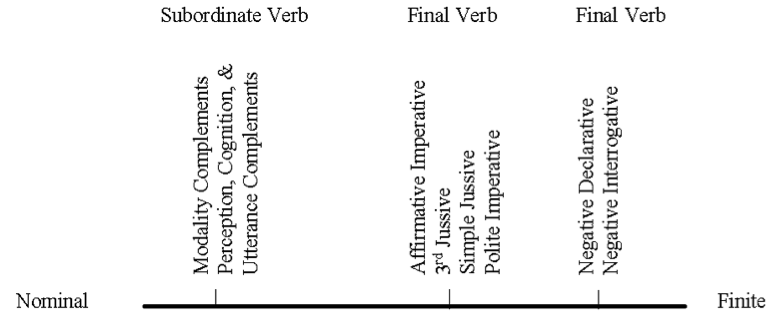
\includegraphics[width=\textwidth]{figures/MAhlandFig1.png}	
\caption{A nominal-finite continuum of infinitive verb stem usage}
\label{fig:1}
\end{figure}
\todo{redraw 2 graphics as vector}

In declarative and interrogative final verbs, infinitive stems are only found in negatives (which always involve the irrealis verbal construction); see \figref{fig:2} (reproduced from \citealt[266]{Ahland2012}).\footnote{The realis and irrealis verb constructions are formed with different item-arrangements in terms of morphology—see \sectref{sec:mahland:3.3}, below. The left-most ellipse in \figref{fig:2} lists features associated only with the realis verb form, while the right-most ellipse lists features associated with the irrealis verb form. The shared center lists those features which are compatible with both realis and irrealis verb forms. Additional verb constructions which do not involved the realis nor the irrealis verb form are listed at the bottom of \figref{fig:2}.} Affirmative realis (non-future) and irrealis (future) verbs require finite stems. Many affirmative imperative and jussive forms require infinitive verb stems, indicated by the boxed section in \figref{fig:2}. The reason for this likely involves differing grammaticalization pathways. There must be a reason why the infinitive stem requirement is only associated with negative constructions that utilize the irrealis verb (regardless of morphological tense marking), with certain imperative and jussive constructions, and with most highly nominalized subordinate verbs. This distribution attests to a nominalized history for these constructions. 
 

\begin{figure}
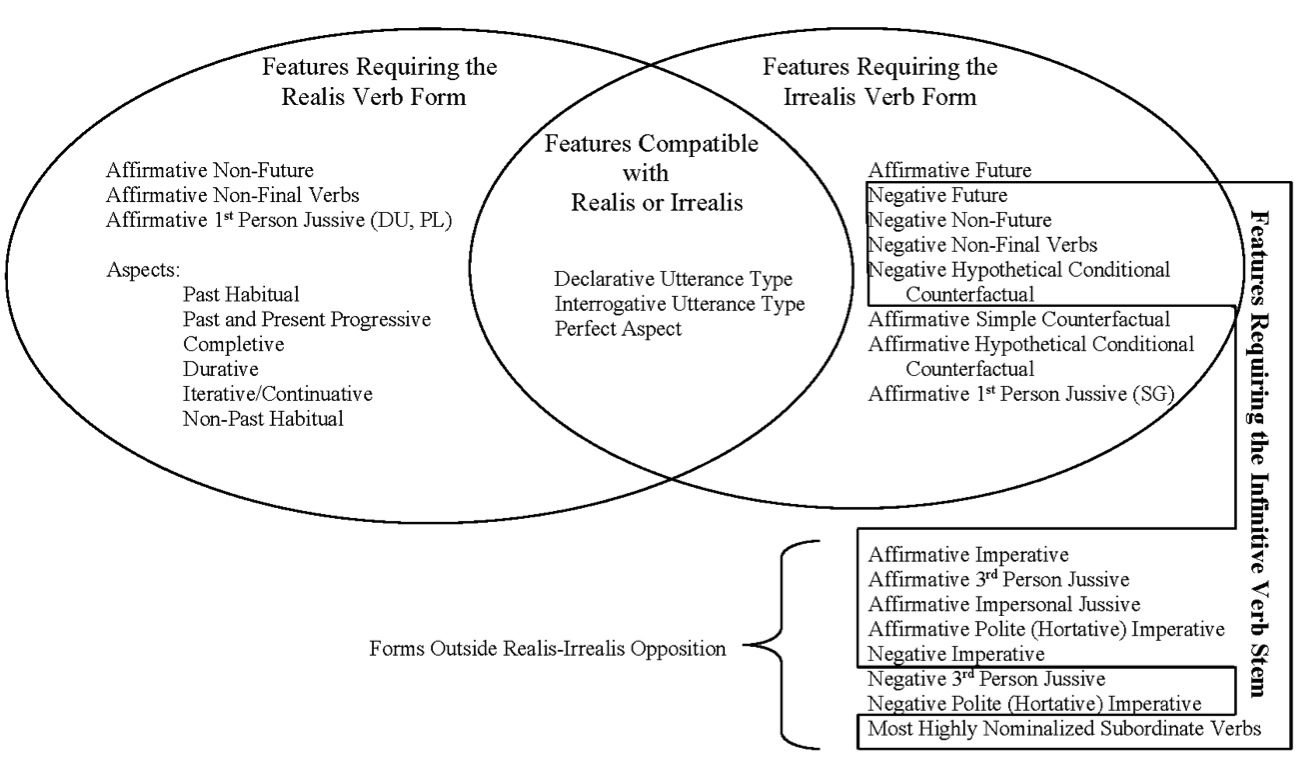
\includegraphics[width=\textwidth]{figures/MAhlandFig2.png}
\caption{The distribution of infinitive verb stems and the intersection with the realis-irrealis opposition}\todo[inline]{Figure 2 is not clear}
\label{fig:2}
\end{figure}
%%make this image on a landscape page?


Before turning to the use of the infinitive verb stems in finite final verbs, use of the finite verb stem is briefly illustrated: affirmative declarative non-future (realis) \REF{ex:mahland:52}, declarative future (irrealis) \REF{ex:mahland:53}, interrogative non-future \REF{ex:mahland:54} and interrogative future \REF{ex:mahland:55} (both irrealis).

\ea\label{ex:mahland:52}
\gll ha-tí-héz-{\downstep}á\\
\textsc{aff-1sg}{}-hit-\textsc{decl} \\
\glt `I hit (it).'
\z

\ea\label{ex:mahland:53}
\gll ha-héz-gà-t-bíʃ-á\\
\textsc{aff}{}-hit-\textsc{fut-1sg-npst:aux-decl} \\
\glt `I will hit (it).'
\z

\ea\label{ex:mahland:54}
\gll tí-héz-àː       /    ha-tí-héz-âː\\
\textsc{1sg}{}-hit-\textsc{intr}   ~  \textsc{aff-1sg}{}-hit-\textsc{intr}\\
\glt `Did I hit (it)?'      `Did I hit (it)?' \\
(expecting an affirmative response)
\z

\ea\label{ex:mahland:55}
\gll héz-gà-t-bíʃ-àː\\
hit-\textsc{fut-1sg-npst:aux-intr}\\
\glt `Will I hit (it)?'
\z

\subsubsection{The negative construction}\label{sec:mahland:3.1.1}

Unlike the affirmative declarative and interrogative examples in \REF{ex:mahland:52}-\REF{ex:mahland:55} which require the finite verb stem, examples \REF{ex:mahland:56}-\REF{ex:mahland:60} illustrate the corresponding negative constructions (non-future and future) which require the use of the infinitive stem.

\ea\label{ex:mahland:56}
\gll hez-á-tí-bíʃ-á\\
hit:\textsc{inf-neg-1sg-npst:aux-decl} \\
\glt `I did not hit (it).'
\z

\ea\label{ex:mahland:57}
\gll hez-á-gà-tí-bíʃ-á\\
hit:\textsc{inf-neg-fut-1sg-npst:aux-decl} \\
\glt `I will not hit (it).'
\z

\ea\label{ex:mahland:58}
\gll hez-á-hì-biʃ-àː\\
hit:\textsc{inf-neg-2sg-npst:aux-intr}\\
\glt `Did you not hit (it)?'
\z

\ea\label{ex:mahland:59}
\gll hez-á-gà-t-bíʃ-àː\\
hit:\textsc{inf-neg-fut-1sg-npst:aux-intr}\\
\glt `Will I not hit (it)?'
\z

Apart from the requirement of the infinitive verb stem, the negative final verbs appear to be fully finite today (e.g. exhibiting a tense distinction and utterance type/speech act marking). 

The organization of the internal morphology of the negative verb in \REF{ex:mahland:56}-\REF{ex:mahland:59} suggests that it developed from a periphrastic structure like \REF{ex:mahland:60}. The bifurcation of negatives into future and non-future constructions appears to be a later development and is discussed in \sectref{sec:mahland:3.3}, following the discussion of the affirmative future's development.
\todo{alignment is off in ex. 60.}
\ea\label{ex:mahland:60}
Hypothesized source for negatives\\
Subordinate structure        Final verb\\
\textsc{inf} stem] + -á \textsc{sub}               \textsc{sbj}{}-Existential verb-\textsc{decl}\\
\gll  hez                {}-á                 tí-           bíʃ      {}-á    \\
  hit\textsc{:inf}          \textsc{{}-neg}            \textsc{1sg}{}-            \textsc{exist}   \textsc{{}-decl} \\
  \glt `I did not hit (it).' ({\textless} I was not hitting.)  (from ex. 56)
  \z
  \todo{alignment between two header rows and example needs to be fixed.}
 
The negative verb appears to have begun as a nominalized complement (an infinitive with a subordinating morpheme that was later reanalyzed as a negative marker) followed by a fully-finite final existential verb with subject prefixes.\footnote{The use of lexical verbs with infinitive stems in auxiliary-headed constructions is quite common cross-linguistically \citep[56]{Anderson2006}.} This periphrastic structure presumably then collapsed into the single verbal word observed today (see \sectref{sec:mahland:3.3}).

\subsubsection{Imperative and jussive utterances}\label{sec:mahland:3.1.2}


As noted in \figref{fig:2}, infinitive stems are also required in certain imperative and jussive constructions. Unlike the other constructions we have seen, however, the infinitive stems in \REF{ex:mahland:61}-\REF{ex:mahland:63} are used in affirmative constructions. 

\ea\label{ex:mahland:61}
\gll hez-í\\
hit:\textsc{inf-2sg:imp}\\
\glt `Hit (it)ǃ'
\z

\ea\label{ex:mahland:62}
\gll há-hez-í\\
\textsc{impr}{}-hit\textsc{:inf-2sg:imp}\\
\glt `Hit (it)ǃ' (polite)
\z

\ea\label{ex:mahland:63}
\gll há-hez-t-í-nè\\
\textsc{impr}{}-hit:\textsc{inf-juss-3-npst:aux}\\
\glt `Let it hit (it).'
\z

Infinitive and jussive forms do not carry tense or aspect marking in Northern Mao—which all other final verb forms do carry. That said, however, infinitive forms do all carry subject markers which also serve to indicate the utterance type. These verbs, like all other final verbs, indicate the end of a sentence, unless a coordinating conjunction is employed.

With respect to the jussive construction in \REF{ex:mahland:63}, the /ne/ form in the impersonal jussive \REF{ex:mahland:63} is a recognizable copula in Northern Mao \REF{ex:mahland:64} \citep[463]{Ahland2012}.

\ea\label{ex:mahland:64}
\gll wèːŋk'           nè\\
be.open\textsc{:inf}    be.\textsc{npst}\\
\glt `It is open.' 
\z

The /há-/ impersonal prefix in the impersonal jussive construction in \REF{ex:mahland:63}, as well as on the polite imperative in \REF{ex:mahland:62}, may derive from an old demonstrative which gave rise to a 3\textsuperscript{rd} person marker in other Mao languages \citep[206]{Bender2000}, \citep[245-246]{Ahland2012}, \citep{Ahland2015};\footnote{Reflexes can be found throughout the Mao subgroup and the form is still used in Seezo /hán/ \citep{Mengistu2015}; a reflex is also found in Hozo /ʔá/ \textsc{3sg} masculine \citep{Kassa2014}.} the /-t/ \textsc{juss} is likely derived from or related to the /-(i)t/ relativizer (reanalyzed as a jussive construction marker). The hypothesized source construction in \REF{ex:mahland:65} illustrates the demonstrative + relativized infinitive stem (nominal) as a predicate, which is then followed by a copula. 

\ea\label{ex:mahland:65}
Hypothesized source for jussive construction\\
Modified Headless Relative (nominal)  Final verb\\
\glll \textsc{dem}   [[\textsc{inf}]          + -(i)t~\textsc{rel]}                \textsc{sbj-} Copula\\
              há   {\db}{\db}hez              ~   {}-t                    í-   nè     \\
      \textsc{dem} {\db}{\db}hit\textsc{:inf} ~ \textsc{{}-rel}                3-   \textsc{cop}\\
\glt `It is that which hit.' {>} `Let it hit (it).' (similar to ex. 63)
\todo[inline]{check alignment of this example}
\z

The jussive source in \REF{ex:mahland:65} is represented as having been a headless relative clause (i.e. a nominal). The fact that the relativized stem is in the infinitive form suggests that the demonstrative would very likely not have been an argument of the relative clause. Perhaps the /há/ demonstrative was a modifier of the relativized predicate.

The imperative construction exhibits the only final verb in the language which uses an infinitive stem where there is no other recognizable verb stem.\footnote{ In the impersonal jussive, for example, the /nè/ form itself appears to derive from a copula verb.} It is not clear if an older verbal stem atrophied and disappeared or if this represents a different grammaticalization pathway. 

The imperative construction \REF{ex:mahland:66} is unique in NM in that both the affirmative and negative polarities require the infinitive verb stem.  

\ea\label{ex:mahland:66}
\gll hez-áʃ-í\\
hit:\textsc{inf-neg-2sg:imp}\\
\glt `Do not hit (it)ǃ'
\z

\subsection{Relativization and the past progressive construction}\label{sec:mahland:3.2}

The progressive constructions involve periphrastic constructions where lexical verbs are followed by auxiliary verbs. In the past progressive, the lexical verb obligatorily carries the /-(i)t/ relativizer \REF{ex:mahland:67}-\REF{ex:mahland:68}.

\ea\label{ex:mahland:67}
\gll hí-kí-èt                 ha-tí-mí-t          bitè\\
\textsc{3sg}{}-come-\textsc{ti:nf}   \textsc{aff-1sg}{}-eat-\textsc{rel}   \textsc{pst:aux} \\
\glt `I was eating when s/he came.'
\z

\ea\label{ex:mahland:68}
\gll ha-jéːts'-ìt    bitè\\
\textsc{aff}{}-run-\textsc{rel}   \textsc{pst:aux}\\
\glt `S/he was running.'
\z

In fact, in the past progressive construction there are two cases of historical relativization. The past copula form /bitè/ is itself a relativization of the existential verb /biʃ/ (cf. \citealt[318; 461-462]{Ahland2012}, and the highlighted form in \REF{ex:mahland:69}): /biʃ -t/ {>} /bi-t/ \textsc{exist-rel}. In \REF{ex:mahland:69}'s matrix clause, the cleft with present meaning requires no copula (i.e. a zero copula); while in \REF{ex:mahland:70}, the past copula is used (in this instance, the form /bitè/ is not a functional auxiliary). 

\ea\label{ex:mahland:69}
\gll [[nà-àt       \textbf{bi-t}]\textsubscript{RC}               ʃak'-è]\textsubscript{NP} Ø    [tí-pí-t-ìʃ-é]
\\
{\db}{\db}here-\textsc{loc}    \textsc{exist}:\textsc{inf-rel}    goat-\textsc{tv}    be.\textsc{pres}  {\db}\textsc{1sg}{}-kill-\textsc{rel-sbj-tv}\\
\glt `It is the goat that was here that I killed.'
\z

\ea\label{ex:mahland:70}
\gll [[nà-àt    \textbf{bi-t}]\textsubscript{RC}             ʃak']\textsubscript{ NP}    \textbf{bitè}    ({\textless} bi-t-è)      [tí-pí-t-ìʃ-é]\\
{\db}{\db}here\textsc{{}-loc}   \textsc{exist:inf-rel}   goat    be.\textsc{pst}  ({\textless} \textsc{exist:inf-rel-tv})  {\db}\textsc{1sg}{}-kill-\textsc{rel-sbj-tv}\\
\glt `It was the goat that was here that I killed.'
\z

The past copula form is a frozen form like all other Northern Mao copulas today \citep[465]{Ahland2012}.

Interestingly, the non-past progressive construction appears to have developed via a slightly different pathway: 1) there is no hint of relativization and 2) the auxiliary is the non-relativized existential \REF{ex:mahland:71}. 

\ea\label{ex:mahland:71}
\gll toːlo   ha-tí-mí         biʃ-á   \\
now   \textsc{aff-1sg}{}-eat    \textsc{npst:aux-decl} \\
\glt `I am eating now.'
\z
In sum, the non-past progressive shows no overt morphological indication of nominalization in its history. But the past progressive construction does and may have developed from a nominal + nominal predication (relativization + relativization), as in \REF{ex:mahland:72}: 

\ea\label{ex:mahland:72}
Hypothesized source for past progressive\\
Relative clause      Relative clause \\{}
\glll [\textsc{sbj-}finite] + -(i)t~\textsc{rel}   [\textsc{exist inf}] + -(i)t~\textsc{rel}  + -\textsc{tv}      \\
         ha-tí-mí                  ~  {}-t                    bi ~ -t-è\\
\textsc{aff}-\textsc{1sg}-eat      ~  {}-\textsc{rel}     \textsc{exist:inf} ~ \textsc{-rel-tv}\\
\glt `I was eating.'
\todo[inline]{Please check the alignment of this example}
\z

Alternatively, it could be that the /bitè/ auxiliary was already grammaticalized as a past copular form $-$ it is difficult to know whether the form was still functioning as a relative clause at the time the past progressive developed. Either way, the lexical verb was clearly expressed, as it is today, within a preceding (nominalized) relative clause.\footnote{As noted in \sectref{ex:mahland:2.2}, the use of subject marking on relativized verbs requires the use of the finite stem even though the clause is still nominalized via the relativizer.}

\subsection{The irrealis future verb construction}\label{sec:mahland:3.3}

Northern Mao's final future (irrealis) verb also developed from a nominal subordinate clause. The lexical verb was marked with a subordinator and was followed by a final existential verb (an \textsc{aux}{}-headed construction; see \citealt[39ff]{Anderson2006}). The subordinator was then reanalyzed as a future tense suffix. The entire periphrastic construction collapsed phonologically, resulting in a complex final verb with contained internal relics of subordinator and related subject marking. (See \citealt{Ahland2014b} for further details.) 

\tabref{tab:mahland:5} and example \REF{ex:mahland:73} illustrate the structure of the realis verbal word. 

\newcommand{\parenbox}[2]{$\Big(\begin{array}{l}\text{#1}\\\text{#2}\end{array}\Big)$}

\begin{table}
\caption{Realis verb item-arrangement (from \citealt[3]{Ahland2014b})}
\label{tab:mahland:5}
\fittable{
\begin{tabular}{ll || l || ll || lllll}
% \lsptoprule
\multicolumn{2}{c||}{\textbf{Inflectional prefixes}} & \textbf{Finite}

 \textbf{stem} & \multicolumn{2}{c||}{\textbf{Derivational suffixes}} & \multicolumn{5}{c}{\textbf{Inflectional suffixes}}\\
&&&&&&&&\\[-.4em]
\hline
&&&&&&&&\\
(Affirmative) &
 \parenbox{Subject}{prefix} &
  &
 \parenbox{Valence}{decreasers} &
 (Applicative)\index{derivational suffixes!applicative} &
 (Perfect)\index{aspect!perfect} &
 \parenbox{Non-}{singular} &
 \parenbox{Past}{habitual} & 
 (Hearsay)\index{Declarative!Hearsay} &
 \parbox{1.5cm}{Utterance\\type}\index{Mood / Utterance Type}\\
% \lspbottomrule
\end{tabular}
}
\end{table}

\ea\label{ex:mahland:73}
\gll kwalla    ha-tí-jéːts'-{\downstep}á \\
yesterday  \textsc{aff-1sg}{}-run\textsc{{}-decl} \\
\glt `I ran yesterday.'
\z

\tabref{tab:mahland:6} and example \REF{ex:mahland:74} illustrate the structure of the irrealis verbal word. 

\begin{table}
\caption{Irrealis future affirmative item-arrangement (from \citealt[4]{Ahland2014b})}
\label{tab:mahland:6}
\fittable{
\begin{tabular}{l || l || ll || lllllll}
\textbf{Inflectional prefix} & \textbf{Finite stem} & \multicolumn{2}{c||}{\textbf{Derivational suffixe}s} & \multicolumn{7}{c}{\textbf{Inflectional suffixes}}\\ 
&&&&&&&&\\[-.4em]
\hline
&&&&&&&&\\
(Affirmative) &
  &
 \parenbox{Valence}{decreasers} &
 (Applicative)\index{derivational suffixes!applicative} &
 (Perfect)\index{aspect!perfect} &
 \parenbox{Non-}{singular} &
 Future suffix &
 Subject suffix &
 Auxiliary &
 (Hearsay)\index{Declarative!Hearsay} &
 Utterance type\index{Mood / Utterance Type}\\ 
\end{tabular}
}
\end{table}

Example \REF{ex:mahland:74} illustrates the irrealis verbal word. 


\ea\label{ex:mahland:74}
\gll hátsʼá    ha-jéːts'-gà-t-bíʃ-á     \\
tomorrow  \textsc{aff}{}-run-\textsc{fut-1sg-npst:aux-decl} \\
\glt `I will run tomorrow.'
\z

The primary differences between the realis and the irrealis verbal words involve the position of subject markers (prefixes on realis verbs and suffixes on irrealis verbs), as well as the presence of an auxiliary verb on the irrealis verbal word. 

In order to understand the history of the irrealis verb, it is important to note that today's future tense suffix /-gà/ is similar to a purposive subordinate\index{subordination} marker /-gàʃ/ found on purpose adverbials \REF{ex:mahland:75}, as well as on some complements \REF{ex:mahland:76} (cf. \sectref{sec:mahland:2.3} above). 

\ea\label{ex:mahland:75}
\gll [kàːl-là     mí]-gàʃ  tí-kí-ti-á\\
  porridge-\textsc{obj}    eat-\textsc{purp}  \textsc{1sg}{}-come-\textsc{pf-decl} \\
  \glt `I have come to eat porridge.'
\z

\ea\label{ex:mahland:76}
\gll mì-gàʃ-nà             ha-tí-ts'éːl-{\downstep}á \\
  eat:\textsc{inf-comp-obj}  \textsc{aff-1sg-}finish-\textsc{decl}   \\
  \glt `I finished eating.'
\z

It has been argued that purpose clauses are “intrinsically future-oriented” \citep[43]{Schmidtke-Bode2009}. In fact, purpose clauses and their matrix verbs are an attested source of future constructions across many of the world's languages (p.181). These complex constructions undergo grammaticalization such that the matrix verb becomes an auxiliary.\footnote{\citet[263-75]{BybeeEtAl1994} note how purpose clauses and concepts such as `intention' and `desire' are “compatible or harmonic” with the grammaticalization of future tense.} This is what appears to have taken place in NM's irrealis future verb construction. 

Before discussing the reconstructed source construction for NM's irrealis future verb, it should be noted that the future tense suffix /-gà/ appears to have been /-gàm/ at an earlier stage in its development. Internal irregularities found in the future relative clause\index{subordination!relative clauses} preserve what appears to be an older [m], i.e. /-gàm/ as in \REF{ex:mahland:77} (cf. \citealt[10]{Ahland2014b}).

\ea\label{ex:mahland:77}
\gll ha-tí-kí-gàm-b-t\\
  \textsc{aff-1sg}{}-come-\textsc{fut-npst:aux-rel}\\\glt `that I will come'
\z

This old [m] is a significant part of the development of the irrealis future verb: the [m] has impacted the subject marking paradigm by intruding into 3\textsuperscript{rd} person and \textsc{2sg} marking in all constructions where today's future tense marker is found; see the shaded cells of \tabref{tab:mahland:7}. 

\begin{table}
\caption{Free pronouns and subject marking on final verbs \citep[7]{Ahland2014b}}
\label{tab:mahland:7}
\begin{tabularx}{\textwidth}{llp{1.5cm}Xp{3.5cm}}
\lsptoprule

\multicolumn{2}{X}{ Free pronouns} &  Realis prefixes &  Irrealis non-future\newline (\textsc{neg}) suffixes &  Irrealis future \newline (\textsc{aff} and \textsc{neg}) suffixes\\
\midrule 
 \textsc{1sg} & \itshape tí-jé & \itshape tí- & \itshape {}-tí & \itshape {}-\'{t}\\
 \textsc{1du} & \itshape han-é & \itshape hań- & \itshape {}-ń & \itshape {}-ń\\
 \textsc{1pl} & \itshape hambèl-è & \itshape ha\`{m}- & \itshape {}-\`{m} & \itshape {}-\`{m}\\
 \textsc{2sg} & \itshape hì-jè & \itshape hì- & \itshape {}-hì & \itshape {}-èm \\
 \textsc{2du} & \itshape háw-é & \itshape háw- & \itshape {}-\'{w}   &  - \'{} (H Tone)\\
 \textsc{2pl} & \itshape hàwèl-è & \itshape hàw- & \itshape {}-\`{w} &  - \`{} (L Tone)\\
 \textsc{3sg} & \itshape íʃ-è & \itshape Ø- & \itshape {}-Ø- & \itshape {}-\`{m}\\
 \textsc{3du} & \itshape íʃ-kuw-e & \itshape Ø-   /-and/ & \itshape {}-Ø-   /-and/ & \itshape {}-\`{m}     /-and/\\
 \textsc{3pl} & \itshape íʃ-kol-è & \itshape Ø-   /-and/ & \itshape {}-Ø-   /-and/ & \itshape {}-\`{m}    /-and/\\
\lspbottomrule
\end{tabularx}
\end{table}

The distribution of the intrusive [m] relative to subject marking is discussed following introduction of the reconstructed source construction. 

As noted above, complex constructions of the type purpose clause + matrix verb are an attested source of future tense constructions. The presence of a relic subordinator positioned before an old subject-marked existential ({>} auxiliary verb) in the irrealis future construction suggests that irreality (and future temporality) was expressed through a periphrastic construction like the reconstruction in (78) (adapted from \citealt[11]{Ahland2014b}).\footnote{Since affirmative future irrealis verbs exhibit only finite verb stems today, the /-gàm/ form must have attached only to the finite form. Today, however, both finite and infinitive stems can take the /-gàʃ/ subordinator, depending on the degree of finiteness of the subordinate clause (cf. \citealt[629]{Ahland2012}).}

\ea\label{ex:mahland:78}
Hypothesized source for future irrealis\\
Subordinate\index{verbs!subordinate} structure   Final verb\\
\gll  kí{}-gàm        ${\emptyset}${}-bíʃ-{\downstep}á\\
  come-\textsc{sub/purp}    \textsc{3sg-exist-decl} \\
  \glt Reconstructed meaning: `S/he is in order to come.'\\
  (Reconstructed effective force: `S/he intends to come.') 
  \z
  
  The old purpose subordinator /{}-gàm /was reanalyzed as a future tense marker. Its final [m] was lost before all initial consonants (except for [h]) on the following subject marker (probably as the entire phrase collapsed into a verb) \REF{ex:mahland:79}-\REF{ex:mahland:80}. The motivation for such a loss could have been consonant cluster simplification. Certainly three-consonant sequences of this sort in NM are not attested. 

\ea\label{ex:mahland:79}
\gll ha-kí-gà\textbf{{}-t}{}-bíʃ-á \\
\textsc{aff}{}-come-\textsc{fut-1sg-npst:aux-decl} \\
\glt `I will come.'
\z

\ea\label{ex:mahland:80}
\gll ha-kí-gà\textbf{{}-n}{}-bíʃ-á \\
\textsc{aff}{}-come-\textsc{fut-1du-npst:aux-decl} \\
\glt `We (dual) will come.'
\z

In the instances where [m] was not lost due to consonant cluster simplification, it became associated with subject person marking \REF{ex:mahland:81}-\REF{ex:mahland:82}.

\ea\label{ex:mahland:81}
\gll ha-kí-gà-\textbf{m}{}-bìʃ-á   \\
\textsc{aff}{}-come-\textsc{fut-3-npst:aux-decl} \\
\glt `S/he will come.'
\z

\ea\label{ex:mahland:82}
\gll ha-kí-g\textbf{{}-èm}{}-bìʃ-á  \\
\textsc{aff}{}-come-\textsc{fut-2sg-npst:aux-decl} \\
\glt `You (singular) will come.'
\z

These facts suggest that the nominal history of the irrealis future verb impacted not only the verbal construction itself, but also the subject marking paradigm.\footnote{This new, altered subject marking paradigm (with the intrusive [m] from the old subordinator) was even extended into new verbal constructions. Today's purpose / complement subordinator /-gàʃ/ perhaps similarly lost the old [m] as a result of cluster simplification before the initial consonant of a following relational noun / postposition /-ʃal/ `way' (cf. \citealt[14]{Ahland2014b}).}  This impact includes the subject markers found on the negative future verb, which also shows the same intrusive [m] interference as the affirmative future (\tabref{tab:mahland:6}; and \citealt[385]{Ahland2012}). 

After the reanalysis of the /-gàm/ form (from subordinator {>} \textsc{fut} suffix) and the formation of the new subject markers, the future tense marker, along with the intrusive [m] in the subject marking, was analogically extended to the negative periphrastic construction \REF{ex:mahland:60}, resulting in two distinct forms: a negative future and negative non-future. The negative non-future was left unchanged. 

If the analysis of the /-á/ negative marker deriving from a subordinator is accurate, there would have been no need for another subordinator such as /-gàm/ (before its reanalysis) on the lexical infinitive form in the negative source construction. This supports the hypothesis that the extension took place after reanalysis. Also, the morphological differences between the negative future and non-future verb forms suggest that the collapse of the non-future periphrastic construction to a single verbal word occurred after the future/non-future distinction developed. While the negative future matches the affirmative future in subject marking and auxiliary patterns (compare \REF{ex:mahland:82} with \REF{ex:mahland:83}), the negative non-future construction exhibits irregularities: an unreduced \textsc{1sg} marker \REF{ex:mahland:84}, an unexpected downstep on the declarative suffix \REF{ex:mahland:84}-\REF{ex:mahland:85}, and an altogether different negative suffix and copular auxiliary for 3rd person forms \REF{ex:mahland:86} (see \citealt[384-384]{Ahland2012} for complete details). 

\ea\label{ex:mahland:83}
\gll ki-á\textbf{{}-}g\textbf{{}-èm}{}-bìʃ-á     \\
come:\textsc{inf-neg-fut-2sg-npst:aux-decl} \\
\glt `You (singular) will not come.'
\z

\ea\label{ex:mahland:84}
\gll ki-á\textbf{{}-}\textbf{tí}{}-bíʃ-{\downstep}á  \\
come:\textsc{inf-fut-1sg-npst:aux-decl} \\
\glt `I didn't come.'
\z

\ea\label{ex:mahland:85}
\gll ki-á\textbf{{}-hi}\textbf{\`{}}{}-bìʃ-{\downstep}á  \\
come:\textsc{inf-fut-2sg-npst:aux-decl}\\
\glt `You (singular) didn't come.'
\z

\ea\label{ex:mahland:86}
\gll ki-wé-jà\\
come:\textsc{inf-neg-cop}\\
\glt `S/he did not come.'
\z

\section{Final considerations}\label{sec:mahland:4}


%%start here
The NM data provide additional support to the typological and historical claim that fully-finite constructions can derive from nominalized structures \citep{Gildea1993, Heine1993, Anderson2006, Anderson2011, DeLancey2011}. In fact, coherent explanation of NM's synchronic, finite final verb structures cannot be achieved without positing a nominal history for the negative declarative and interrogative constructions, imperatives, jussives, past progressives, and irrealis future tense constructions. Apart from such a historical analysis, various irregularities would escape explanation: why is it that some constructions require infinitive verb stems? Why do forms that clearly resemble subordinators (purpose markers and relativizers) appear internal to verbal word-forms? And, why should fused copulas and existentials occur in forms that now function as finite final verbs? 


Givón has noted that in languages which place complements (including clauses) immediately adjacent to verbs, co-lexicalization and clause-union can result \citep[74]{Givon2009}; this is the pattern that is seen repeatedly in the NM developments above. Within the languages of Ethiopia, historically nominal sources for finite structures are by no means limited to the OV pattern. Both VO and OV languages provide clear evidence of old nominalizations embedded in what are today finite structures. In Gumuz (Nilo-Saharan), which exhibits a predominantly VO pattern, the future tense construction derives from a nominalized purpose construction, with the old /mà-/ nominalizer still present in the new finite construction \citep[444]{CAhland2012}. Nominal sources of now-finite verbs are also commonly found in Amharic (Ethiopian-Semitic) as well, where finite perfect verb forms carry nominal possessive suffixes, positioned before an existential ({>} auxiliary) \citep[387]{Leslau1995}.  

\section*{\textbf{Acknowledgments}}

This research was funded in part through a Documenting Endangered Languages grant from the National Science Foundation (\#0746665) under the direction of Doris Payne. This work would not have been possible without the support of the Benishangul-Gumuz Culture Office in Asosa, the support of the Mao communities in Bambassi and Diddessa, especially Ato Yasin Ibrahim, Ato Mamo Shimagele, and Ato Tefera Ibrahim and the support of the Department of Linguistics at Addis Ababa University. I would also like to thank the editors and two anonymous reviews for their helpful comments and suggestions. Of course, any errors are my own. 

\section*{\textbf{Abbreviations}}

Where two abbreviations are combined to form a complex gloss for a single form, the two are joined with a colon (e.g. \textsc{npst:aux}, non-past auxiliary form). 
\bigskip


\begin{tabularx}{.45\textwidth}{lX} 
1 & first person\\
2 & second person\\
3 & third person\\
\textsc{aff}     & affirmative\\
\textsc{aux}     & auxiliary\\
\textsc{comp}     & complementizer\\
\textsc{cop}     & copula\\
\textsc{decl}     & declarative\\
\textsc{def}     & definite\\
\textsc{du}     & dual\\
\end{tabularx}
\begin{tabularx}{.45\textwidth}{lX} 
\textsc{exist}     & existential \\
\textsc{fut}     & future \\
\textsc{gen}     & genitive\\
\textsc{h}     & H tone\\
\textsc{hrsy}     & hearsay\\
\textsc{imp}     & imperative\\
\textsc{impr}     & impersonal\\
\textsc{inf}     & infinitive\\
\textsc{intr}     & interrogative\\
\textsc{juss}     & jussive\\
\end{tabularx}

\begin{tabularx}{.45\textwidth}{lX} 
\textsc{l}     & L tone\\
\textsc{loc}     & locative\\
\textsc{m}     & M tone\\
\textsc{neg}     & negative\\
\textsc{nf}      & non-final\\
\textsc{np}     & noun phrase\\
\textsc{npst}     & non-past\\
\textsc{nsg}     & non-singular (dual/plural)\\
\textsc{obj}     & object case\\
\textsc{pass}     & passive \\
\textsc{pf}     & perfect\\
\textsc{pl}     & plural\\
\end{tabularx}
\begin{tabularx}{.45\textwidth}{lX} 
\textsc{pres}     & present \\
\textsc{prox}     & proximal\\
\textsc{pst}     & past \\
\textsc{purp}     & purposive\\
\textsc{rc}     & relative clause\\
\textsc{rel}     & relativizer\\
\textsc{sbj}     & subject case\\
\textsc{sg}     & singular\\
\textsc{source}   & source oblique\\
\textsc{ss}     & same-subject\\
\textsc{sub}    & subordinate\\
\textsc{ti}     & temporally-integrated\\
\textsc{tv}    & terminal vowel\\
\end{tabularx}


 

\printbibliography[heading=subbibliography,notkeyword=this]



\end{document}